\documentclass[11pt,
  letterpaper,
  openany,
  toc=bibliography,
  idxtotoc,
  bookmarks]{labbook}

\usepackage[utf8]{inputenc}
\usepackage[T1]{fontenc}
\usepackage[spanish]{babel}

\usepackage[margin=2.5cm]{geometry}
\usepackage{microtype}
\usepackage{graphicx}
\usepackage{amsmath,amssymb}
\usepackage{csquotes}
\usepackage{booktabs}
\usepackage{enumitem}
\usepackage{authblk}
\usepackage[spanish]{cleveref}
\usepackage[dvipsnames]{xcolor}
\usepackage{pgfplotstable}
\usepackage{siunitx}
\usepackage{subcaption}
\usepackage{multirow}

\pgfplotsset{compat=1.18}
\pgfkeys{/pgf/number format/1000 sep={\,}}

\AtBeginDocument{\decimalpoint}
\renewcommand{\arraystretch}{1.2}
\sisetup{group-digits=true,
  group-separator={\,},
  separate-uncertainty}

\usepackage[backend=biber,style=numeric]{biblatex}
\addbibresource{./references-pre-project.bib}

\usepackage{pdfbase}
\pdfinfo{
  /Title (Electron Beam)
  /Author (Sebastián Rodríguez, Laura Torres, Julián Ávila)
  /Creator (LaTeX with labbook class)
}

\title{\textbf{Rayo de Electrones} \\
Bitácora de Laboratorio}
\author{Sebastian Rodríguez \and Laura Torres \and Julian Avila}
\affil{Universidad Distrital Francisco José de Caldas}
\date{}

\begin{document}

\maketitle

\tableofcontents

\chapter{Análisis del Montaje Experimental}
\label{sec:analisis_montaje}

El montaje experimental presenta simetrías notables que determinan los
posibles efectos a observar.

Independientemente de la dirección relativa de los campos magnéticos
generados por cada par de bobinas coaxiales, el sistema exhibe una
simetría de reflexión respecto a los planos $xz$, $yz$ y $xy$.
Esto se debe a la simetría axial intrínseca de las bobinas y a su disposición
simétrica respecto al origen.

Además, si ambos pares de bobinas operan a la misma frecuencia, se
obtiene una simetría rotacional de $\pi/2$ en el plano $yz$.
En el caso general de frecuencias distintas, esta se reduce a una simetría de
rotación de $\pi$.
Estas simetrías son fundamentales para la construcción de los modelos teóricos
y la simplificación de los cálculos.
Por tanto, se espera que los patrones observados en la pantalla reflejen estas
mismas simetrías.

\section{Modelos Clásicos con Álgebra Geométrica}
\label{sec:modelo_clasico}

Se postula que la dinámica del electrón está gobernada por la fuerza de
Lorentz. En el régimen de bajas energías
($\qty{4.1}{\kilo\eV} \ll \qty{511}{\kilo\eV}$),
los efectos relativistas son despreciables. De esta forma, la ecuación
diferencial a resolver es la \cref{eq:lorentz-force}, donde $-e$ y $m$ son
la carga y la masa del electrón, respectivamente. Los campos son el
vector eléctrico $\boldsymbol{E}$ y el bivector magnético $\boldsymbol{B}$.

La ecuación se presenta en el formalismo del álgebra geométrica
$\mathcal{C}\ell_{3}(\mathbb{R})$. El término
$\langle \dot{\boldsymbol{x}} \boldsymbol{B} \rangle_{1}$ denota la
proyección de grado-1 (vector) del producto geométrico, el cual
corresponde a la fuerza magnética.
%
\begin{equation}
	m \ddot{\boldsymbol{x}} = -e \left( \boldsymbol{E}
	+ \langle \dot{\boldsymbol{x}} \boldsymbol{B} \rangle_{1} \right)
	\label{eq:lorentz-force}
\end{equation}

Para todos los modelos se asume que no existe interacción
electrón-electrón. Aplicando las ecuaciones de Maxwell homogéneas,
%
\begin{gather}
	\label{eq:faraday-gauss}
	\nabla \boldsymbol{E} = -\partial_t \boldsymbol{B},
	\\
	\label{eq:no-monopoles}
	\langle \nabla \boldsymbol{B} \rangle_{3} = 0,
\end{gather}
%
se deduce la existencia de un potencial vectorial magnético
$\boldsymbol{A} \in \mathcal{C}\ell^1$ (\emph{i.e} $A = \langle A \rangle_{1}$)
tal que $\boldsymbol{B} = \nabla \wedge \boldsymbol{A} \equiv \langle\nabla
\boldsymbol{A}\rangle_{2}$.
Sustituyendo en la ley de Faraday, se obtiene el campo eléctrico inducido
en la ausencia de un potencial escalar ($\phi=0$):
%
\begin{equation}
	\nabla \boldsymbol{E} = -\partial_t \langle\nabla \boldsymbol{A}\rangle_{2}
	\implies
	\left\langle \nabla (\boldsymbol{E} + \partial_t \boldsymbol{A})
	\right\rangle_{2} = 0
	\implies
	\boldsymbol{E} = - \partial_t \boldsymbol{A}.
	\label{eq:induced-E}
\end{equation}

\subsection{Modelo I: Campo Magnético Espacialmente Uniforme}
\label{ssec:campo_uniforme}

En una configuración de bobinas de Helmholtz, donde las corrientes fluyen
en la misma dirección, se genera un campo magnético aditivo y
notablemente uniforme en la región central entre ellas. Como primera
aproximación, se postula que el campo magnético $\boldsymbol{B}$ es
espacialmente uniforme y depende únicamente del tiempo.

El campo total es la superposición de los campos generados por cada par
de bobinas. En el formalismo de álgebra geométrica, este bivector es:
\begin{gather}
	\boldsymbol{B}(t) = B_2(t) e_{31} + B_3(t) e_{12},
	\label{eq:B_field_uniform}
	\\
	B_i(t) = \left( \frac{4}{5} \right)^{\frac{3}{2}}
	\frac{\mu_0 n I_{i}(t)}{R} =: B_0 I_i(t),
	\label{eq:B_field_magnitude}
\end{gather}
%
donde $\mu_0$ es la permeabilidad del vacío, $n$ el número de vueltas de
cada bobina, $R$ su radio, y $I_i(t)$ la corriente de alimentación. El
subíndice $i \in \{2, 3\}$ denota el eje cartesiano correspondiente.

Dada la no unicidad del potencial vectorial magnético $\boldsymbol{A}$, se
adopta el \emph{gauge simétrico}:
%
\begin{equation}
	\boldsymbol{A}(\boldsymbol{x}, t) = \frac{1}{2}
	\langle \boldsymbol{x} \boldsymbol{B}(t) \rangle_{1}.
	\label{eq:symmetric_gauge}
\end{equation}
%
Esta elección satisface correctamente la condición
$\langle \nabla \boldsymbol{A} \rangle_{2} = \boldsymbol{B}$.
El campo eléctrico inducido se deriva de
$\boldsymbol{E} = - \partial_t \boldsymbol{A}$, resultando en:
%
\begin{equation}
	\boldsymbol{E}(\boldsymbol{x}, t) = - \frac{1}{2} \langle \boldsymbol{x}
	\, \partial_t \boldsymbol{B}(t) \rangle_{1}.
	\label{eq:E_induced_uniform}
\end{equation}

\subsubsection{Análisis de la Dinámica del Campo Magnético}
\label{sssec:dinamica_b}

La estructura temporal del campo magnético, descrita en la
\cref{eq:B_field_uniform}, determina la naturaleza de la fuerza ejercida
sobre el electrón. Para visualizar esta dinámica, se analiza la
evolución del vector dual al bivector magnético,
$\boldsymbol{B}^* = \boldsymbol{B}e_{123}^{-1}$. Esto equivale a realizar
una gráfica paramétrica de la componente $B_3(t)$ en función de $B_2(t)$.

Cuando las corrientes $I_2(t)$ e $I_3(t)$ son sinusoidales, la
trayectoria resultante es una \emph{figura de Lissajous}. La morfología de
esta figura depende críticamente de la razón de frecuencias,
$\omega_2/\omega_3$, y del desfase, $\phi$, entre ambas señales.

En este experimento se utilizaron también señales cuadradas, generando
dinámicas distintas. Para dos señales cuadradas, la trayectoria traza un
perímetro rectangular, con transiciones que dependen de la relación de
frecuencias. La combinación de una señal sinusoidal y una cuadrada
produce una trayectoria confinada entre dos segmentos rectos, conectados
por arcos sinusoidales.

La \cref{fig:B_fields} ilustra estas tres configuraciones para una razón
de frecuencia de 3:1 y un desfase nulo, mostrando la rica variedad de
campos magnéticos temporales que se pueden generar.

\begin{figure}[htbp!]
	\centering
	\begin{subfigure}{0.32\linewidth}
		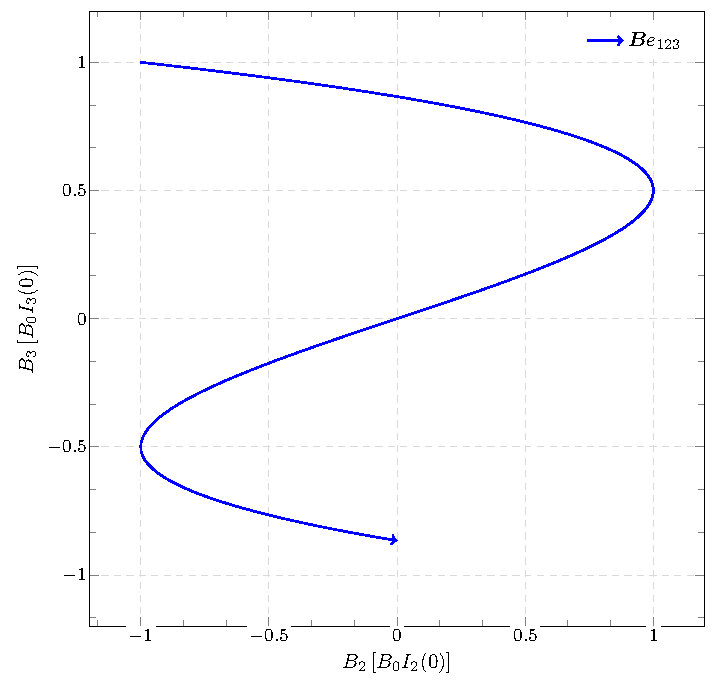
\includegraphics[width=\linewidth]{../Figures/Uniform-Field/B-sin-sin.pdf}
		\caption{Señales sinusoidales.}
		\label{fig:b_sin_sin}
	\end{subfigure}
	\hfill
	\begin{subfigure}{0.32\linewidth}
		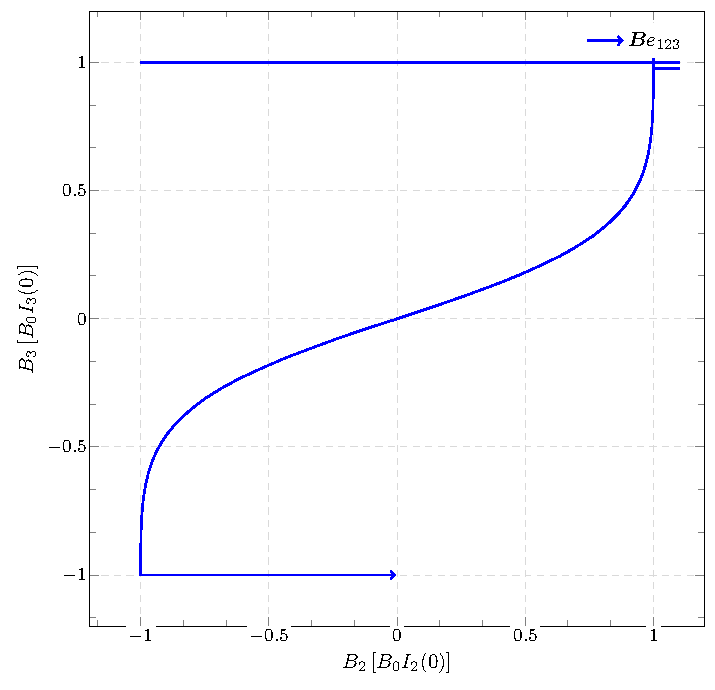
\includegraphics[width=\linewidth]{../Figures/Uniform-Field/B-square-square.pdf}
		\caption{Señales cuadradas.}
		\label{fig:b_sqr_sqr}
	\end{subfigure}
	\hfill
	\begin{subfigure}{0.32\linewidth}
		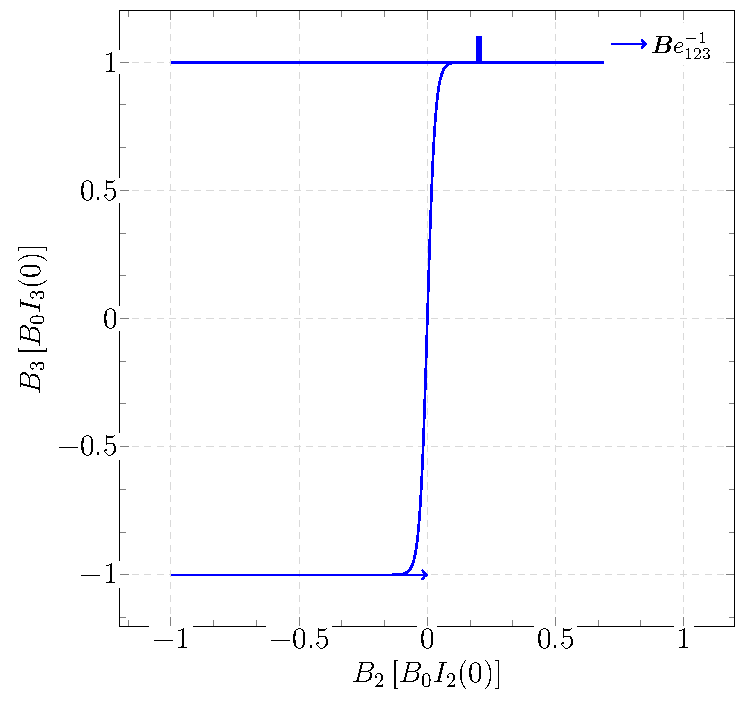
\includegraphics[width=\linewidth]{../Figures/Uniform-Field/B-sin-square.pdf}
		\caption{Señal sinusoidal y cuadrada.}
		\label{fig:b_sin_sqr}
	\end{subfigure}
	\caption{Evolución del vector de campo magnético $\boldsymbol{B}^*$ en
		el plano $yz$ para distintas formas de onda de la corriente. Se
	muestra una razón de frecuencias de 3:1 y un desfase $\phi=0$.}
	\label{fig:B_fields}
\end{figure}

\subsubsection{Análisis del Campo Eléctrico Inducido}
\label{sssec:dinamica_e}

El campo eléctrico inducido $\boldsymbol{E}$ depende de la tasa de cambio
del campo magnético, $\partial_t \boldsymbol{B}$. Su magnitud es, por
ende, proporcional a la frecuencia de las corrientes de alimentación.
A continuación, se cuantifica su efecto en comparación con el campo
magnético para las condiciones específicas del experimento.

La razón entre las magnitudes de las fuerzas eléctrica y magnética es:
%
$$
\frac{|\boldsymbol{F}_E|}{|\boldsymbol{F}_B|} \approx
\frac{|\boldsymbol{E}|}{v |\boldsymbol{B}|}
$$
%
Para una señal sinusoidal, $|\boldsymbol{E}| \approx R \omega |\boldsymbol{B}|$,
donde $R$ es el radio de las bobinas, $\omega$ la frecuencia angular y $v$
la velocidad del electrón. La razón de fuerzas es entonces $\approx R\omega/v$.

Con los parámetros del montaje, se tiene:
%
\begin{itemize}
	\item Una frecuencia $f \approx \qty{50}{\hertz}$, que implica una frecuencia
		angular $\omega = 2\pi f \approx \qty{314}{\radian\per\second}$.
	\item Una energía cinética de $\qty{4.1}{\kilo\eV}$, que corresponde a una
		velocidad del electrón de $v \approx 0.1c$.
	\item Un radio de bobinas $R$ del orden de $\qty{6.2}{\centi\meter}$.
\end{itemize}
%
Sustituyendo estos valores se obtiene:
%
$$
\frac{|\boldsymbol{F}_E|}{|\boldsymbol{F}_B|} \approx \frac{R\omega}{v}
\approx 10^{-7}
$$
%
Este resultado numérico, de orden $10^{-7}$, confirma de manera
contundente que la fuerza magnética es aproximadamente \emph{diez millones} de
veces mayor que la fuerza eléctrica. Por lo tanto, es una aproximación
justificada considerar que la dinámica es gobernada
exclusivamente por el campo magnético, omitiendo el término de
$\boldsymbol{E}$ en el modelo.


\subsection{Modelo II: Campo a partir de la Ley de Biot-Savart}
\label{ssec:modelo_biot_savart}

En este modelo, se abandona la aproximación de campo uniforme para calcular
el campo magnético de forma más fundamental. Se utiliza la ley de
Biot-Savart para cada espira de las bobinas.

Se considera una única espira circular de radio $R$ en el plano inferior
del par de bobinas del eje $z$, ubicado en $z = -R/2$. Su geometría se
parametriza por el vector $\boldsymbol{l}_1(\theta)$:
%
\begin{equation}
	\boldsymbol{l}_1(\theta) = R \cos(\theta) e_1 + R \sin(\theta) e_2
	- \frac{R}{2} e_3.
\end{equation}
%
El campo magnético bivectorial que esta espira genera en un punto
arbitrario $\boldsymbol{r} = x_1 e_1 + x_2 e_2 + x_3 e_3$ está dado por la
ley de Biot-Savart, integrada sobre el lazo cerrado:
%
\begin{equation}
	\boldsymbol{B}_1(t, \boldsymbol{r}) = \frac{\mu_0 N I_1(t)}{4 \pi} \oint
	\frac{\mathrm{d}\boldsymbol{l}_1 \wedge (\boldsymbol{r} - \boldsymbol{l}_1)}
	{|\boldsymbol{r} - \boldsymbol{l}_1|^3},
	\label{eq:biot_savart_bivector}
\end{equation}
%
donde $N$ es el número de vueltas de la bobina y $I_1(t)$ es la corriente
que circula por ella.

El campo de la segunda bobina del par, ubicada coaxialmente en $z = +R/2$,
se deduce por simetría. Si la corriente $I_2(t)$ en la bobina superior
circula en la misma dirección que $I_1(t)$ (configuración Helmholtz),
la relación de simetría es distinta; no obstante, la forma del campo
resultante es bien conocida por su alta uniformidad en la región
central, para la cual existen soluciones analíticas estándar.

Por otro lado, si se considera una configuración anti-Helmholtz (corrientes
opuestas), el sistema presenta una simetría de inversión. En este caso, el
campo de la segunda bobina, $\boldsymbol{B}_2$, se relaciona con el de la
primera mediante una reflexión sobre el origen:
%
\begin{equation}
	\boldsymbol{B}_2(t, \boldsymbol{r}) =
	-\boldsymbol{B}_1(t, -\boldsymbol{r}, I_1(t)).
	\label{eq:simetria_inversion_B}
\end{equation}
%
Esta importante simplificación surge de la simetría axial de las bobinas
combinada con la simetría de paridad de la configuración. El campo total
del par de bobinas es entonces la superposición
$\boldsymbol{B}_{\text{par}}(t, \boldsymbol{r}) = \boldsymbol{B}_1 + \boldsymbol{B}_2$.
El mismo análisis se aplica a los otros pares de bobinas a lo largo de los
demás ejes.

\subsubsection{Campo Eléctrico en la Configuración anti-Helmholtz}
\label{sssec:campo_electrico_ah}

Aunque el análisis cuantitativo previo ya justifica la dominancia de la
fuerza magnética, la configuración anti-Helmholtz presenta una propiedad
de simetría que refuerza esta conclusión.

Debido a la simetría axial y de inversión de esta configuración, el
potencial vectorial magnético $\boldsymbol{A}$ es nulo a lo largo del eje
de las bobinas. Como consecuencia directa, el campo eléctrico inducido,
$\boldsymbol{E} = -\partial_t \boldsymbol{A}$, también es cero sobre dicho
eje. Esto implica que en la región central del montaje, la más relevante
para la trayectoria del haz, el efecto del campo eléctrico es aún más
despreciable.

\subsection{Modelo III: Aproximación de Campo Cuadrupolar}
\label{ssec:modelo_cuadrupolar}

El campo generado por un par de bobinas en configuración anti-Helmholtz
puede ser aproximado cerca de su centro por un campo de gradiente lineal,
característico de un cuadrupolo magnético. Al superponer los campos de
varios pares, se obtiene un campo cuadrupolar tridimensional.

Una aproximación lineal para dicho campo es:
%
\begin{equation}
	\boldsymbol{B}(\boldsymbol{r}, t) = b(t)
	\left( - x_1 e_{23} + \frac{1}{2} x_2 e_{31} + \frac{1}{2} x_3 e_{12} \right).
	\label{eq:quadrupole_field}
\end{equation}
%
Este campo satisface la condición de Maxwell $\langle \nabla \boldsymbol{B} \rangle_3 = 0$.
La dependencia temporal del campo se engloba en el coeficiente $b(t)$.

Este tipo de campo de gradiente es la base de las trampas magnéticas.
Cuando las corrientes son tales que el campo apunta hacia el origen, se
crea un pozo de potencial que confina el haz (efecto de \emph{enfoque}).
Inversamente, si el campo apunta hacia afuera, las partículas son
repelidas del centro (\emph{desenfoque}).

Con corrientes alternas, el sistema oscila entre un estado de enfoque y
desenfoque. Esto puede resultar en un confinamiento dinámico neto del
haz, un principio análogo al de las trampas de Paul para partículas
cargadas.



\section{Análisis de la Interacción de Espín}
\label{ssec:modelo_spin}

Hasta ahora, se ha modelado al electrón como una carga puntual clásica. Sin
embargo, el electrón es una partícula cuántica con espín $\frac{1}{2}$, lo
que le confiere un momento dipolar magnético intrínseco $\boldsymbol{\mu}$.
Esta propiedad podría, en principio, dar lugar a una fuerza adicional si el
campo magnético no es uniforme.

El momento magnético del electrón es $\boldsymbol{\mu} = g_s \frac{-e}{2m} \boldsymbol{S}$,
donde $\boldsymbol{S}$ es el vector de espín y $g_s \approx 2$ es el
factor g del electrón. En presencia de un campo magnético con gradiente,
esto genera la \emph{fuerza de Stern-Gerlach}:
%
\begin{equation}
	\boldsymbol{F}_{\text{espín}} = \nabla (\boldsymbol{\mu} \cdot \boldsymbol{B}^*),
	\label{eq:fuerza_spin}
\end{equation}
%
donde $\boldsymbol{B}^*$ es el vector dual al bivector de campo magnético
$\boldsymbol{B}$. A continuación se argumenta por qué esta fuerza es
despreciable en comparación con la fuerza de Lorentz.

\subsection{Comparación de Magnitudes}

En el \emph{Modelo I} (campo uniforme), $\nabla \boldsymbol{B}^* = 0$ por
definición, por lo que $\boldsymbol{F}_{\text{espín}}$ es idénticamente
nula. En los modelos más realistas con gradientes de campo (II y III), se
puede estimar la razón entre la fuerza de espín y la fuerza de Lorentz:
%
$$
\frac{|\boldsymbol{F}_{\text{espín}}|}{|\boldsymbol{F}_{\text{Lorentz}}|}
\approx \frac{|\nabla (\boldsymbol{\mu} \cdot \boldsymbol{B}^*)|}
{|e\boldsymbol{v} \times \boldsymbol{B}^*|}
\approx \frac{\mu_B |\nabla \boldsymbol{B}^*|}{e v |\boldsymbol{B}^*|}
$$
%
donde $\mu_B = e\hbar/2m$ es el magnetón de Bohr. Suponiendo que el campo
varía en una escala de longitud $L \sim R$ (el radio de las bobinas),
entonces $|\nabla \boldsymbol{B}^*| \approx |\boldsymbol{B}^*|/R$. La razón se
simplifica a:
%
$$
\frac{|\boldsymbol{F}_{\text{espín}}|}{|\boldsymbol{F}_{\text{Lorentz}}|}
\approx \frac{\hbar}{2m v R} \approx 10^{-11}
$$
%
Este cálculo, usando los parámetros del montaje, demuestra que la fuerza
de Lorentz es aproximadamente once órdenes de magnitud mayor que la
fuerza derivada del espín, justificando plenamente su omisión.

\subsection{Efecto de la Precesión de Larmor}

Independientemente de la estimación anterior, existe un segundo argumento.
En presencia de un campo $\boldsymbol{B}$, el momento magnético
$\boldsymbol{\mu}$ del electrón no permanece fijo, sino que experimenta un
torque que lo hace precesar alrededor de la dirección de $\boldsymbol{B}^*$
a la \emph{frecuencia de Larmor}, $\omega_L$.

Dado que la fuerza $\boldsymbol{F}_{\text{espín}}$ depende de la orientación
instantánea de $\boldsymbol{\mu}$, esta fuerza también oscilará rápidamente.
En el tiempo que tarda el electrón en atravesar una región con gradiente de
campo, su espín habrá completado muchas precesiones. El efecto neto de esta
fuerza oscilante sobre la trayectoria macroscópica se promedia a cero.

Por estas dos razones, es físicamente justificable y computacionalmente
necesario ignorar la interacción del espín para los propósitos de este
estudio, y continuar tratando al electrón como una carga clásica.


\pgfplotstableread[col sep=comma, header=true]{
  i, y_cm_i, m_i
  1, 14.2, 600.8
  2, 28.0, 1216.3
  3, 14.0, 601.8
}\mydata

\pgfplotstableread[col sep=comma, header=true]{
  config, mode, freq1, freq2, freq3
  \multirow{3}{*}{5-1}, 100, 1.2715, 0.8408, 0.0205
  , 010, 0.8308, 0.8308, 0.8308
  , 101, 1.2771, 0.8375, 1.1934
  \multirow{3}{*}{6-1}, 100, 1.3147, 0.8383, 1.2003
  , 010, 0.8415, 0.8415, 0.8415
  , 101, 1.3144, 0.8348, 1.1901
  \multirow{3}{*}{6-2}, 100, 1.3303, 0.8455, 1.2288
  , 010, 0.8378, 0.8378, 0.8378
  , 101, 1.3189, 0.8402, 1.2114
  \multirow{3}{*}{6-4}, 100, 1.3263, 0.8547, 1.3263
  , 010, 0.8498, 0.8498, 0.8498
  , 101, 1.3250, 0.8505, 1.2713
  \multirow{3}{*}{6-6}, 100, 1.3144, 0.8552, 1.3303
  , 010, 0.8519, 0.8519, 0.8519
  , 101, 1.3147, 0.8574, 1.3474
}\datafreq

\pgfplotstableread[col sep=comma, header=true]{
  config, f1, f2, f3
  5-1, 1.1669, 0.8305, 1.2647
  6-1, 1.1669, 0.8343, 1.3120
  6-2, 1.1815, 0.8366, 1.3120
  6-4, 1.2394, 0.8437, 1.3122
  6-6, 1.3100, 0.8513, 1.3356
}\theoric

\pgfplotstableread[col sep=comma, header=true]{
  config, fe, ft, err
  \multirow{3}{*}{5-1}, 0.8308, 0.8305, 0.0361
  , 1.1934, 1.1669, 2.2205
  , 1.2771, 1.2647, 0.9709
  \multirow{3}{*}{6-1}, 0.8415, 0.8343, 0.8556
  , 1.1901, 1.1669, 1.9494
  , 1.3144, 1.3120, 0.1826
  \multirow{3}{*}{6-2}, 0.8378, 0.8366, 0.1432
  , 1.2114, 1.1815, 2.4682
  , 1.3189, 1.3120, 0.5232
  \multirow{3}{*}{6-4}, 0.8498, 0.8437, 0.7178
  , 1.2713, 1.2394, 2.5092
  , 1.3250, 1.3122, 0.9660
  \multirow{3}{*}{6-6}, 0.8519, 0.8513, 0.0704
  , 1.3147, 1.3100, 0.3575
  , 1.3474, 1.3356, 0.8758
}\comparison

\subsection*{Adquisici\'on y Procesamiento de Datos}

Se complet\'o el montaje del sistema de p\'endulos acoplados seg\'un lo
planificado. Se realizaron mediciones de la evoluci\'on angular de cada
p\'endulo utilizando el sensor Cassy.

Se recopilaron un total de 15 series de datos temporales. Estas series
cubren:
\begin{itemize}
  \item Cinco configuraciones experimentales distintas del sistema.
  \item Tres condiciones iniciales diferentes para cada configuraci\'on.
\end{itemize}

Los datos crudos ($\theta_i(t)$ para cada p\'endulo) fueron procesados
mediante un c\'odigo en Python. Los objetivos principales del procesamiento
fueron:
\begin{enumerate}
  \item Generar gr\'aficas de la evoluci\'on angular $\theta_i(t)$ para
    visualizar el comportamiento din\'amico.
  \item Determinar las frecuencias angulares principales de oscilaci\'on
    ($f_i$) para cada p\'endulo en cada serie, aplicando la
    Transformada R\'apida de Fourier (FFT) a los datos temporales.
\end{enumerate}

\subsection*{An\'alisis de Frecuencias Angulares Experimentales}

Las frecuencias angulares principales identificadas se resumen en el
\cref{tab:frequencies}.
\begin{table*}[htbp!]
  \centering
  \caption{Frecuencias angulares principales de oscilaci\'on ($f_i$)
    identificadas para cada p\'endulo, seg\'un la configuraci\'on
  experimental y las condiciones iniciales aplicadas.}
  \label{tab:frequencies}
  \pgfplotstabletypeset[
  every head row/.style={
    before row=\toprule,
    after row=\midrule
  },
  every last row/.style={after row=\bottomrule},
  columns/config/.style={
    string type,
    column name={Configuraci\'on},
  },
  columns/mode/.style={
    string type,
    column name={Condici\'on Inicial},
  },
  columns/freq1/.style={
    column name=$f_1 [\si{\Hz}]$,
    fixed,
    fixed zerofill,
    precision=3,
  },
  columns/freq2/.style={
    column name=$f_2 [\si{\Hz}]$,
    fixed,
    fixed zerofill,
    precision=3,
  },
  columns/freq3/.style={
    column name=$f_3 [\si{\Hz}]$,
    fixed,
    fixed zerofill,
    precision=3,
  },
  every nth row={3}{before row=\midrule},
  columns={config, mode, freq1, freq2, freq3}
  ]{\datafreq} % \datafreq debe apuntar al archivo de datos
\end{table*}

Del an\'alisis preliminar de los valores en \cref{tab:frequencies},
se observan los siguientes patrones:

\textbf{P\'endulo 2 (el m\'as largo):}
\begin{itemize}
  \item Frecuencia angular usual: consistentemente alrededor de
    \qty{0.844}{\Hz}.
  \item Desviaci\'on est\'andar: \num{0.009}. Esto indica una notable
    regularidad en su comportamiento oscilatorio a esta frecuencia.
\end{itemize}

\textbf{P\'endulo 1:}
\begin{itemize}
  \item Se identifican dos agrupaciones principales de frecuencias:
    \begin{itemize}
      \item En torno a \qty{1.311}{\Hz} (desv. est. \num{0.019}).
      \item Cercana a \qty{0.843}{\Hz} (desv. est. \num{0.008}).
    \end{itemize}
\end{itemize}

\textbf{P\'endulo 3:}
\begin{itemize}
  \item Comportamiento similar al p\'endulo 1, con valores ligeramente
    distintos:
    \begin{itemize}
      \item Frecuencias predominantes alrededor de \qty{1.255}{\Hz}
        (desv. est. \num{0.063}).
      \item Frecuencias alrededor de \qty{0.843}{\Hz} (desv. est. \num{0.008}).
    \end{itemize}
  \item Adicionalmente, se detect\'o una frecuencia excepcionalmente baja de
    \qty{0.0021}{\Hz}. Esta se present\'o de manera aislada,
    \'unicamente en la Configuraci\'on 5-1 bajo las condiciones
    iniciales (100).
\end{itemize}

\textbf{Interpretaci\'on inicial:} La aparici\'on de m\'ultiples frecuencias
dominantes para los p\'endulos laterales (1 y 3) sugiere la excitaci\'on
selectiva de diferentes modos normales del sistema. La manifestaci\'on de
estos modos parece depender de la configuraci\'on espec\'ifica de
acoplamiento y de las condiciones iniciales impuestas.

\textbf{An\'alisis detallado de \cref{tab:frequencies}:}
\begin{itemize}
  \item \textbf{Condici\'on inicial (010)} (excitaci\'on \'unica del p\'endulo
    central): Los tres p\'endulos tienden a oscilar con una frecuencia
    dominante com\'un o muy similar, independientemente de la
    configuraci\'on de acoplamiento. Esto podr\'ia indicar la
    excitaci\'on preferente de un modo normal en el que los tres
    p\'endulos participan de manera sincronizada.
  \item \textbf{Otras condiciones iniciales:} El p\'endulo 3 generalmente
    muestra una frecuencia principal inferior a la del p\'endulo 1.
    Una excepci\'on se observa en la configuraci\'on 6-6, donde la
    frecuencia principal del p\'endulo 3 supera a la del p\'endulo 1.
\end{itemize}

\textbf{Factores que influyen en las frecuencias observadas:}
\begin{itemize}
  \item La menor frecuencia caracter\'istica del p\'endulo 2 se atribuye
    principalmente a su mayor longitud y masa (mayor momento de inercia)
    en comparaci\'on con los p\'endulos laterales.
  \item Las diferencias en las frecuencias principales entre los p\'endulos 1 y
    3, y su variaci\'on entre configuraciones, son consecuencia de c\'omo
    los diferentes puntos de acople de los resortes modifican la
    interacci\'on. La altura de fijaci\'on de los resortes influye en los
    torques de acoplamiento y, por ende, en la 'rigidez efectiva
    angular' del acoplamiento. Esto afecta las caracter\'isticas de los
    modos normales.
  \item \textbf{Configuraci\'on 6-6:} Sus puntos de acople espec\'ificos
    parecen facilitar una interacci\'on que favorece un modo donde el
    p\'endulo 3 oscila a una frecuencia mayor que el 1.
  \item \textbf{Frecuencia an\'omala de \qty{0.0021}{\Hz} (P3, Config. 5-1,
    CI (100)):} En esta configuraci\'on, un punto de anclaje del
    resorte est\'a muy pr\'oximo al pivote. Esto resulta en una 'rigidez
    efectiva angular' muy d\'ebil para ciertos patrones de movimiento,
    llevando a frecuencias de oscilaci\'on extremadamente bajas para el
    modo asociado.
  \item \textbf{Configuraci\'on 6-4, CI (100):} Los p\'endulos laterales (1 y 3)
    presentan la misma frecuencia principal. Esto podr\'ia indicar la
    excitaci\'on de un modo normal con alta simetr\'ia en el movimiento
    de los p\'endulos externos.
\end{itemize}

\subsection*{C\'alculo de Frecuencias del Modelo Te\'orico}

Se resolvi\'o el problema de valores propios para el sistema (representado
en forma matricial para obtener las frecuencias te\'oricas de los modos normales
para las cinco configuraciones experimentales.

Los resultados te\'oricos se presentan en el \cref{tab:theoric-freq}.
Se identifican tres frecuencias de modo normal distintas para cada
configuraci\'on, como es de esperar para un sistema con tres grados de
libertad.
\begin{table*}[htbp!]
  \centering
  \caption{Frecuencias te\'oricas de los modos normales ($f_{0i}$)
    calculadas para el sistema, seg\'un la configuraci\'on de
  acoplamiento.}
  \label{tab:theoric-freq}
  \pgfplotstabletypeset[
  every head row/.style={
    before row=\toprule,
    after row=\midrule
  },
  every last row/.style={after row=\bottomrule},
  columns/config/.style={
    string type,
    column name={Configuraci\'on},
  },
  columns/f2/.style={ % Revisar si los nombres f1,f2,f3 son consistentes
    column name=$f_{01} [\si{\Hz}]$, % f01, f02, f03 es más estándar
    fixed,
    fixed zerofill,
    precision=3,
  },
  columns/f1/.style={
    column name=$f_{02} [\si{\Hz}]$,
    fixed,
    fixed zerofill,
    precision=3,
  },
  columns/f3/.style={
    column name=$f_{03} [\si{\Hz}]$,
    fixed,
    fixed zerofill,
    precision=3,
  },
  columns={config, f2, f1, f3} % Asegurar orden correcto de columnas
  ]{\theoric} % \theoric debe apuntar al archivo de datos
\end{table*}

\textbf{Observaciones sobre las frecuencias te\'oricas (\cref{tab:theoric-freq}):}
\begin{itemize}
  \item \textbf{Tendencia general:} Una mayor distancia entre el punto de
    acople del resorte y el pivote del p\'endulo tiende a correlacionarse
    con un aumento en las frecuencias de los modos normales.
  \item \textbf{Valores espec\'ificos:} Se observa con regularidad una
    frecuencia te\'orica cercana a \qty{0.8}{\Hz}. Otras est\'an
    agrupadas en torno a \qty{1.3}{\Hz} y, en algunos casos, pr\'oximas a
    \qty{1.6}{\Hz}.
\end{itemize}

\textbf{Comparaci\'on inicial con datos experimentales:}
\begin{itemize}
  \item Las frecuencias te\'oricas obtenidas, en general, no difieren
    significativamente de los valores experimentales predominantes
    (ver \cref{tab:frequencies}).
  \item \textbf{Excepci\'on notable:} La frecuencia experimental an\'omalamente
    baja de \qty{0.0021}{\Hz} (Config. 5-1, CI (100), P3) no tiene una
    contraparte directa en el espectro te\'orico calculado.
  \item \textbf{Concordancia general:} A pesar de la excepci\'on, la
    concordancia para las dem\'as frecuencias principales sugiere que el
    modelo te\'orico linealizado (basado en peque\~nas oscilaciones)
    aproxima razonablemente el comportamiento din\'amico del sistema.
\end{itemize}

\subsection*{Comparaci\'on Detallada: Frecuencias Experimentales vs. Te\'oricas}

En la \cref{tab:comparison} se presenta una comparaci\'on directa entre las
frecuencias experimentales ($f_\text{ex}$) predominantes (para modos
discernibles) y sus correspondientes frecuencias te\'oricas ($f_\text{te}$).
Se incluye el error relativo porcentual:
$E = \mid \left(1 - \frac{f_\text{te}}{f_\text{ex}}\right) \mid 100\%$.
\begin{table*}[htbp!]
  \centering
  \caption{Comparaci\'on entre las frecuencias experimentales
    predominantes ($f_\text{ex}$) y las frecuencias te\'oricas
    ($f_\text{te}$) para los modos normales, junto con el error
  relativo porcentual.}
  \label{tab:comparison}
  \pgfplotstabletypeset[
  every head row/.style={
    before row=\toprule,
    after row=\midrule
  },
  every last row/.style={after row=\bottomrule},
  columns/config/.style={
    string type,
    column name={Configuraci\'on},
  },
  columns/fe/.style={
    column name=$f_\text{ex} [\si{\Hz}]$,
    fixed,
    fixed zerofill,
    precision=3,
  },
  columns/ft/.style={
    column name=$f_\text{te} [\si{\Hz}]$,
    fixed,
    fixed zerofill,
    precision=3,
  },
  columns/err/.style={
    column name={Error Relativo $[\%]$},
    fixed,
    fixed zerofill,
    precision=3,
  },
  every nth row={3}{before row=\midrule},
  columns={config, fe, ft, err}
  ]{\comparison} % \comparison debe apuntar al archivo de datos
\end{table*}

\textbf{An\'alisis de errores relativos (\cref{tab:comparison}):}
\begin{itemize}
  \item Los errores relativos porcentuales var\'ian considerablemente.
  \item Error m\'as grande observado (sin considerar la frecuencia an\'omala
    de \qty{0.0021}{\Hz}, no incluida aqu\'i): \qty{2.509}{\percent}.
  \item Error m\'as bajo registrado: \qty{0.036}{\percent}.
  \item Estos valores indican que, si bien existen desviaciones, el modelo
    te\'orico predice las frecuencias de los modos normales con un grado
    de precisi\'on generalmente alto para la mayor\'ia de los casos.
\end{itemize}

\subsection*{Visualizaci\'on: Casos Representativos de Oscilaci\'on y Espectros}

Se seleccionaron seis casos del conjunto de datos experimentales como los
m\'as representativos de los diversos comportamientos din\'amicos observados.
Para cada caso, se generaron figuras que muestran:
(a) Evoluci\'on temporal del desplazamiento angular $\theta_i(t)$.
(b) Espectro de amplitudes (FFT) correspondiente.

Estas representaciones gr\'aficas se detallan en las
\cref{fig:111-11,fig:010-51,fig:101-61,fig:010-62,fig:100-66,fig:010-66}.

\begin{figure}[htbp!]
  \centering
  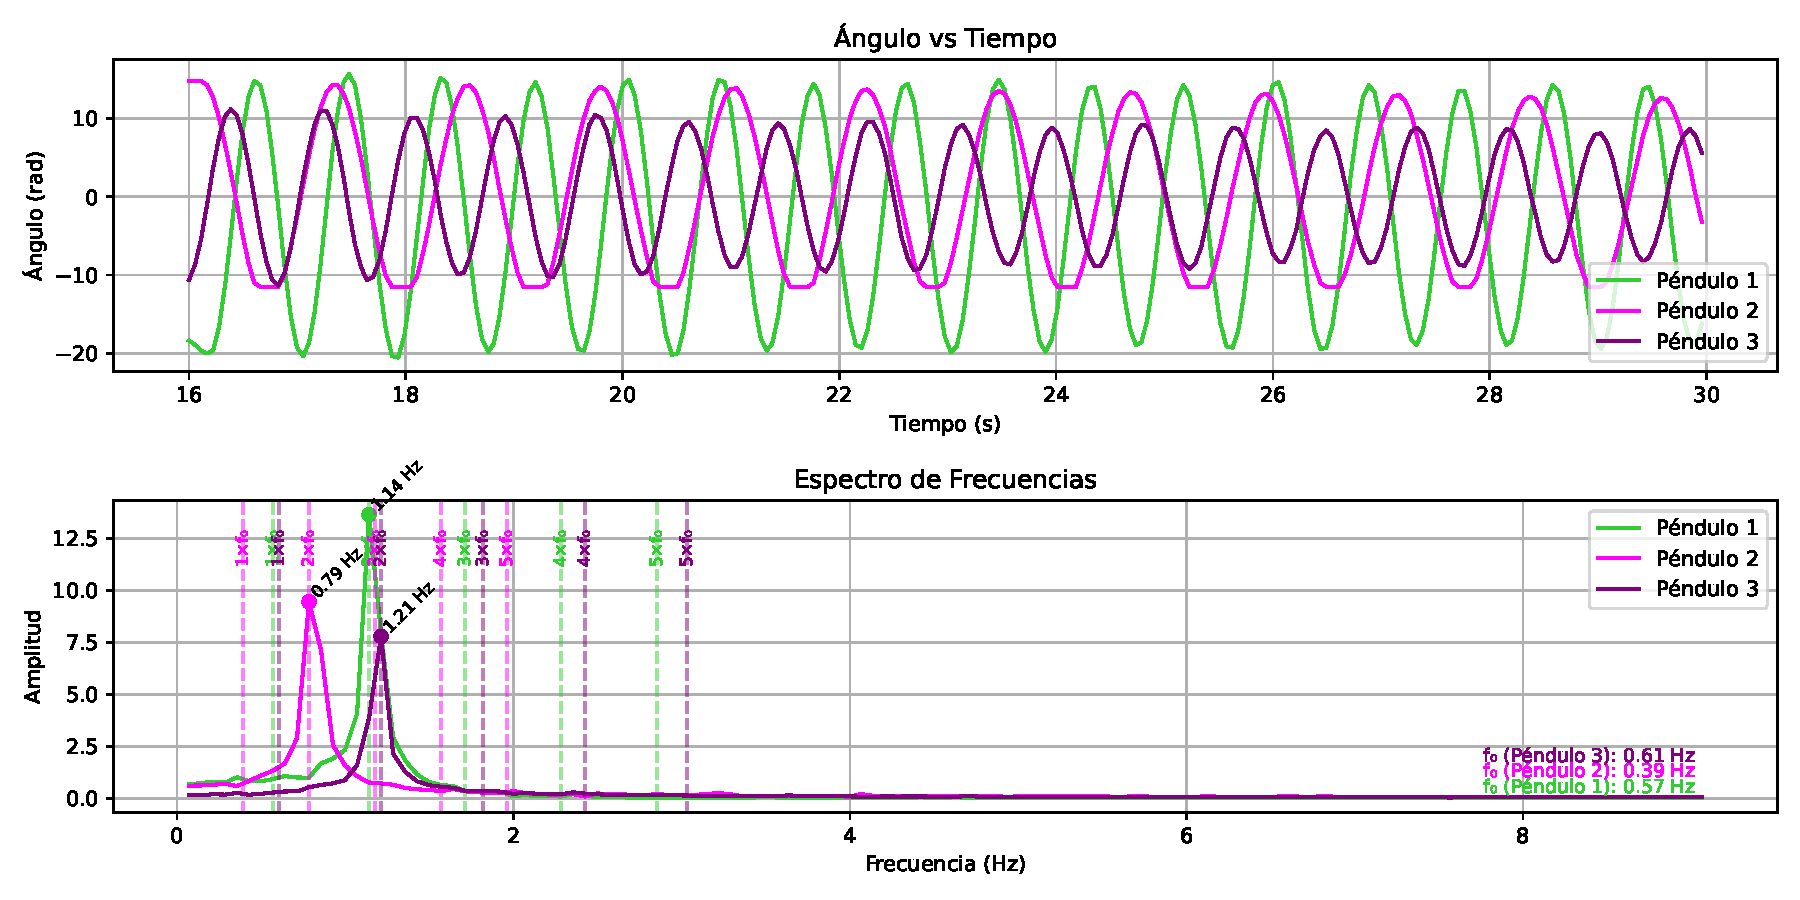
\includegraphics[width=0.8\linewidth]{./Figures/111_11_filtrado.pdf}
  \caption{Evoluci\'on temporal $\theta_i(t)$ y espectro FFT.
  Configuraci\'on 1-1, CI (111).}
  \label{fig:111-11}
\end{figure}

\begin{figure}[htbp!]
  \centering
  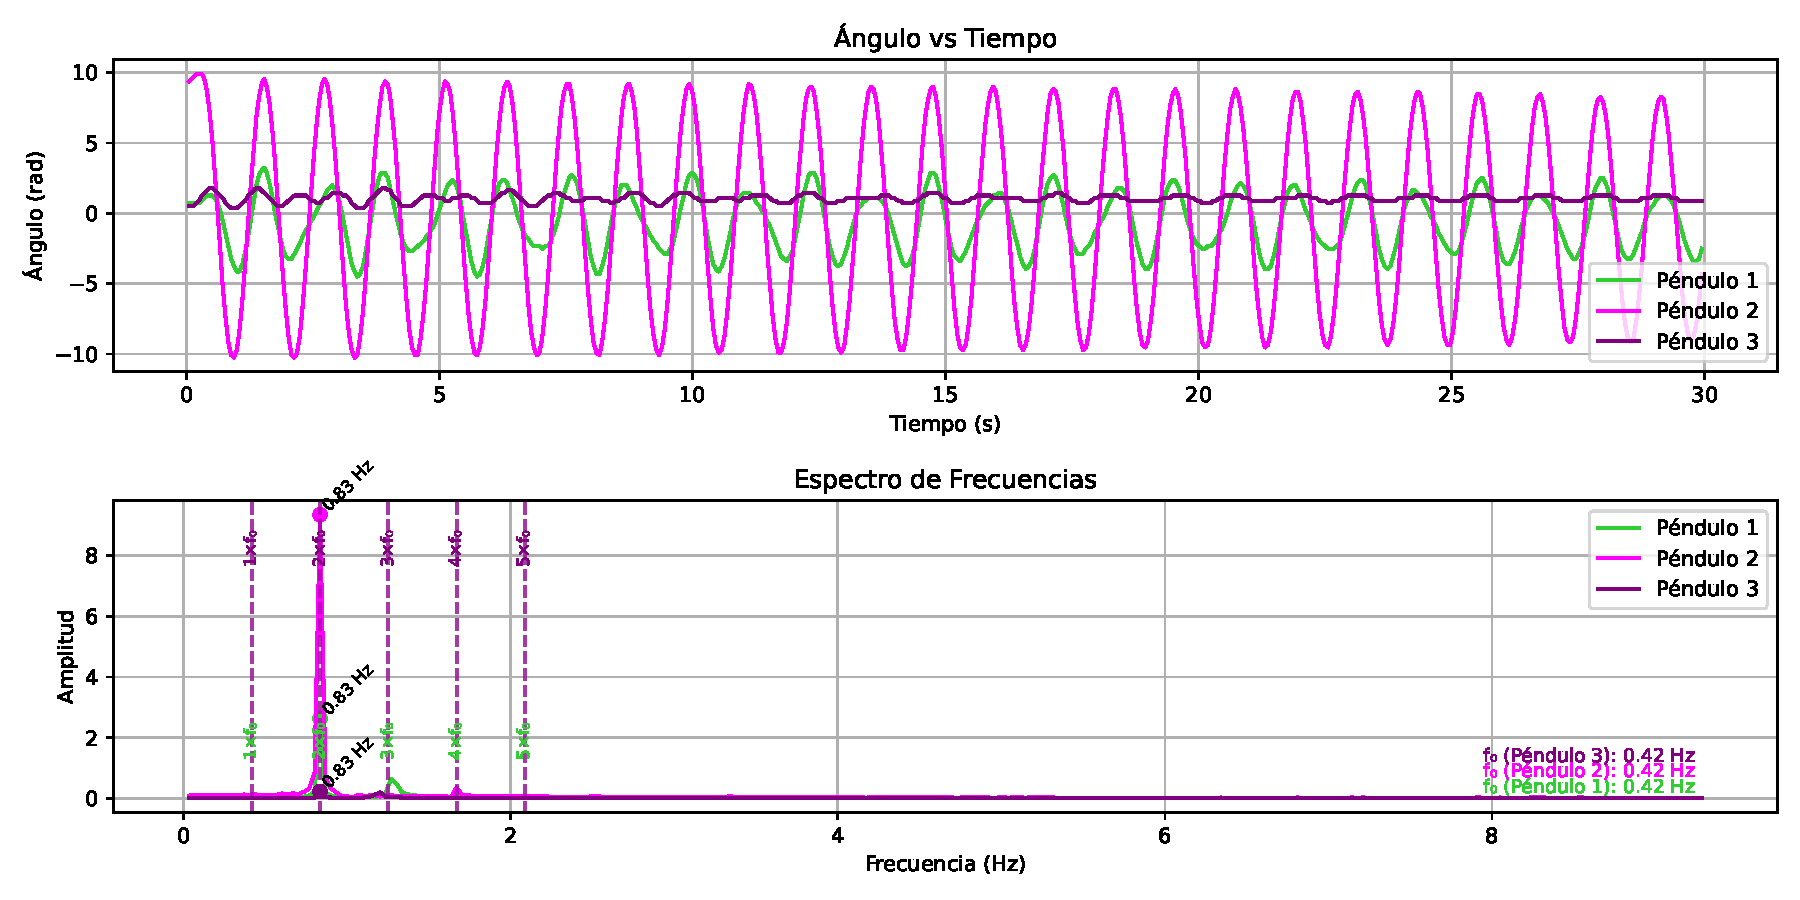
\includegraphics[width=0.8\linewidth]{./Figures/010_15_filtrado.pdf}
  \caption{Evoluci\'on temporal $\theta_i(t)$ y espectro FFT.
  Configuraci\'on 5-1, CI (010).}
  \label{fig:010-51}
\end{figure}

\begin{figure}[htbp!]
    \centering
    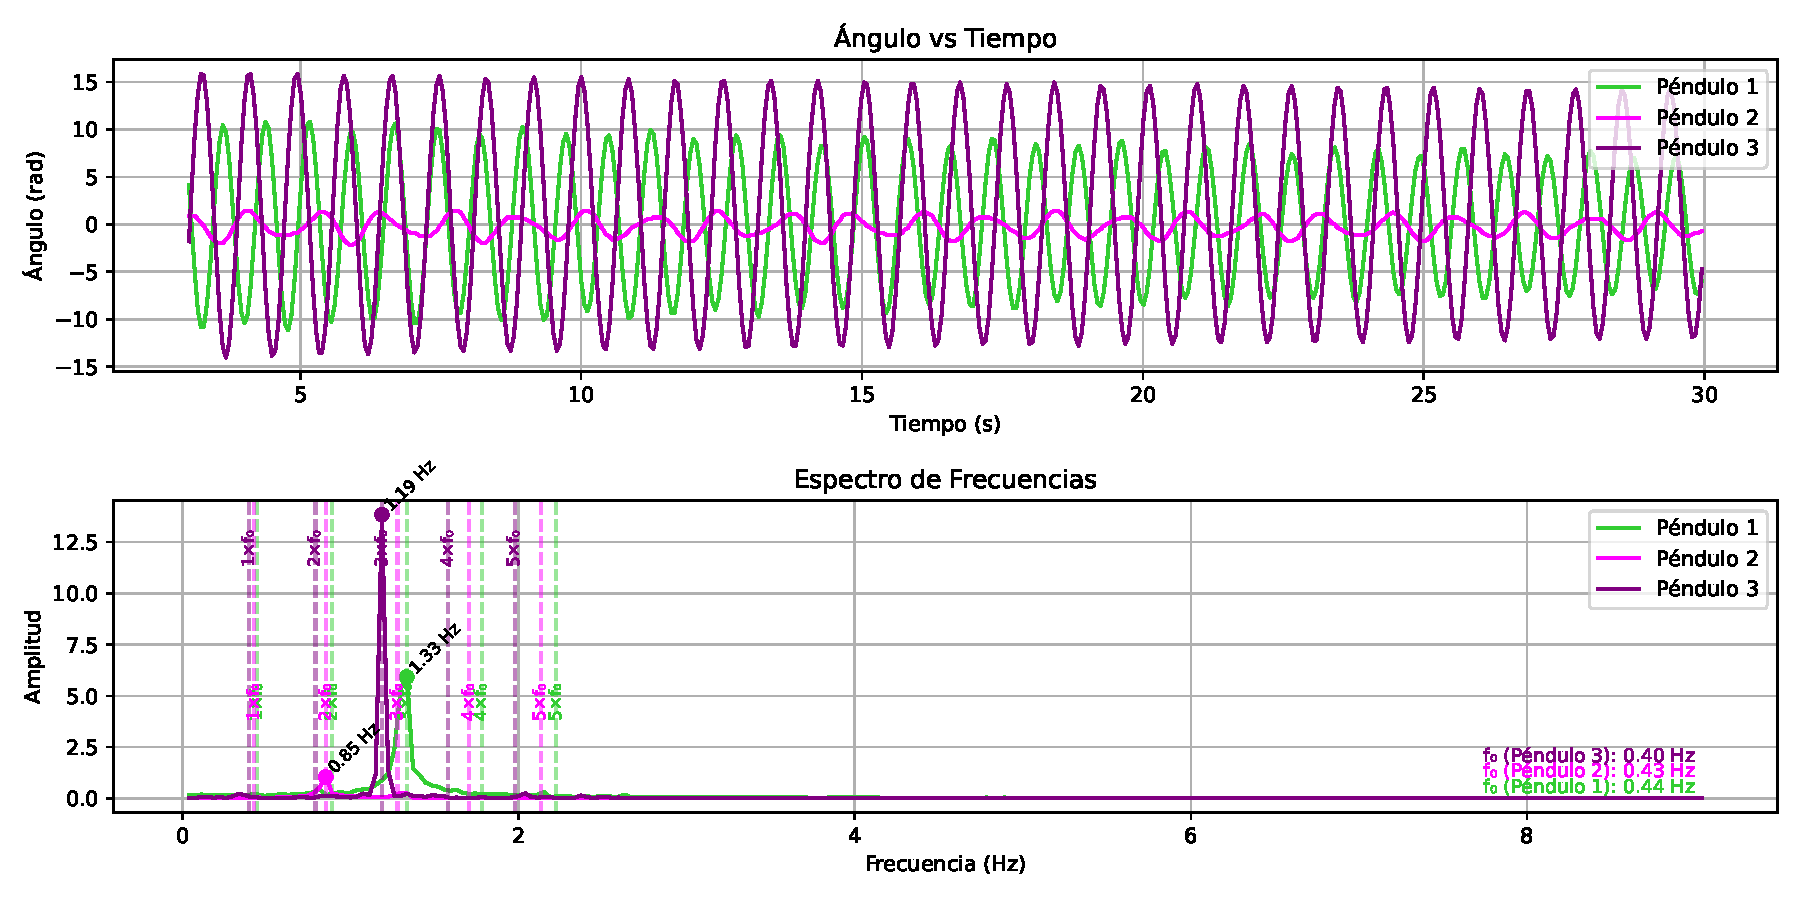
\includegraphics[width=0.8\linewidth]{./Figures/101_16_filtrado.pdf}
    \caption{Evoluci\'on temporal $\theta_i(t)$ y espectro FFT.
        Configuraci\'on 6-1, CI (101).}
    \label{fig:101-61}
\end{figure}

\begin{figure}[htbp!]
    \centering
    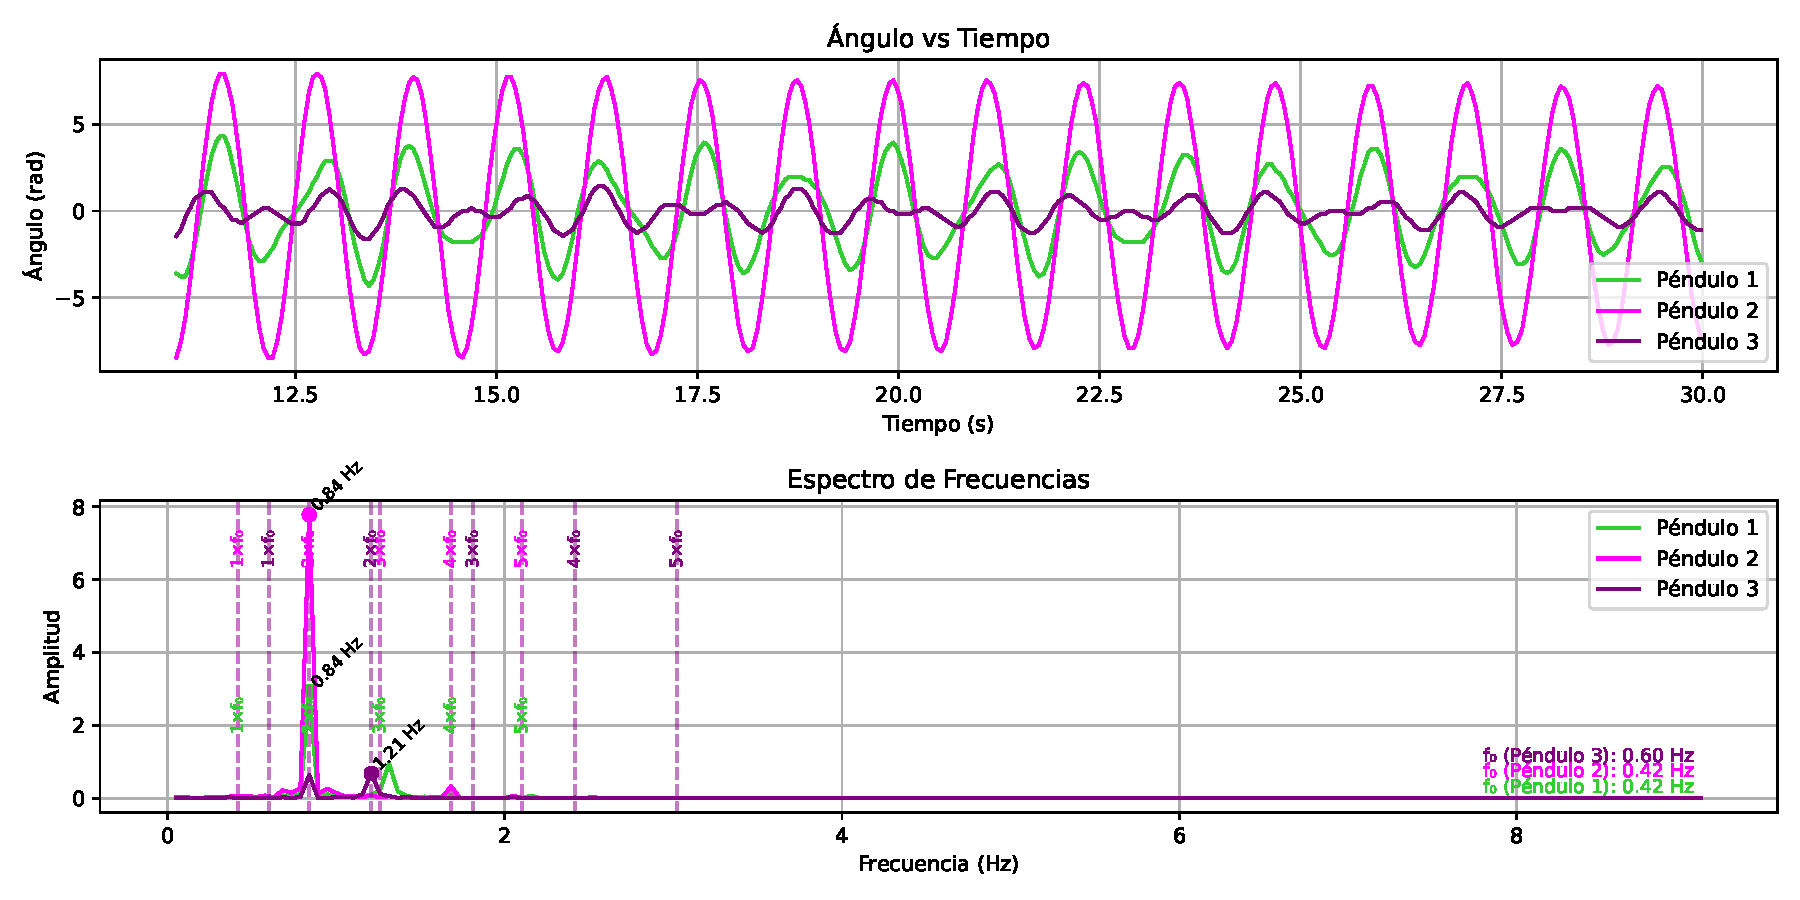
\includegraphics[width=0.8\linewidth]{./Figures/010_26_filtrado.pdf}
    \caption{Evoluci\'on temporal $\theta_i(t)$ y espectro FFT.
        Configuraci\'on 6-2, CI (010).}
    \label{fig:010-62}
\end{figure}

\begin{figure}[htbp!]
    \centering
    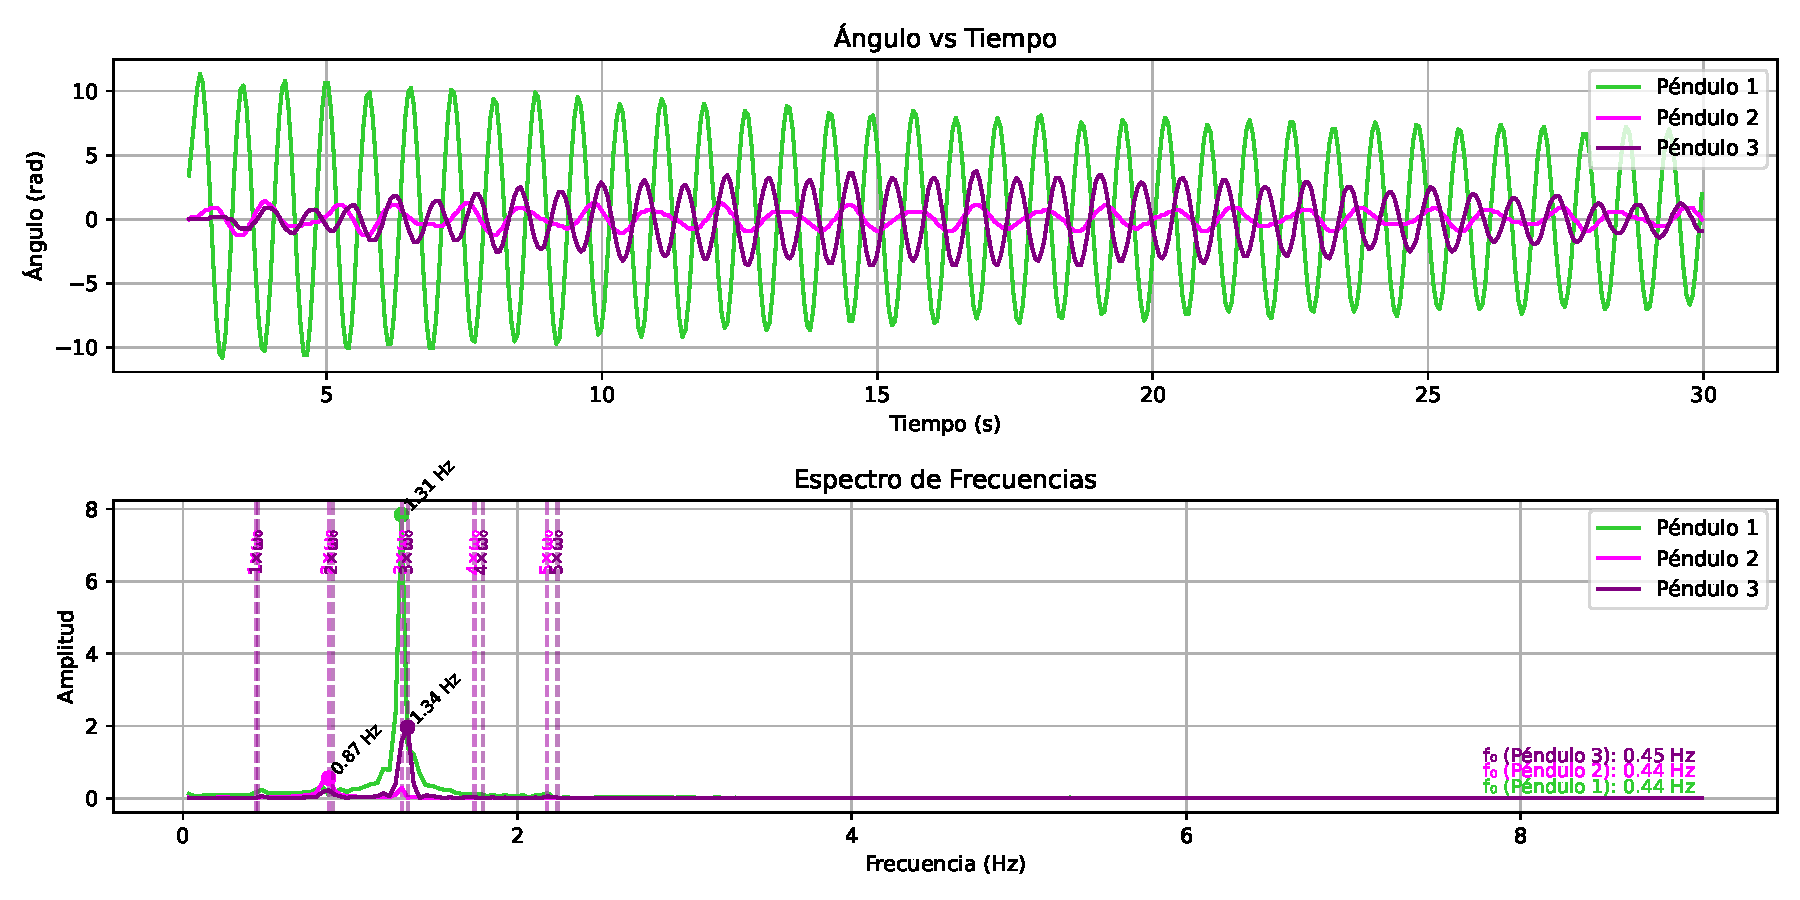
\includegraphics[width=0.8\linewidth]{./Figures/001_66_filtrado.pdf}
    \caption{Evoluci\'on temporal $\theta_i(t)$ y espectro FFT.
        Configuraci\'on 6-6, CI (100).}
    \label{fig:100-66}
\end{figure}

\begin{figure}[htbp!]
    \centering
    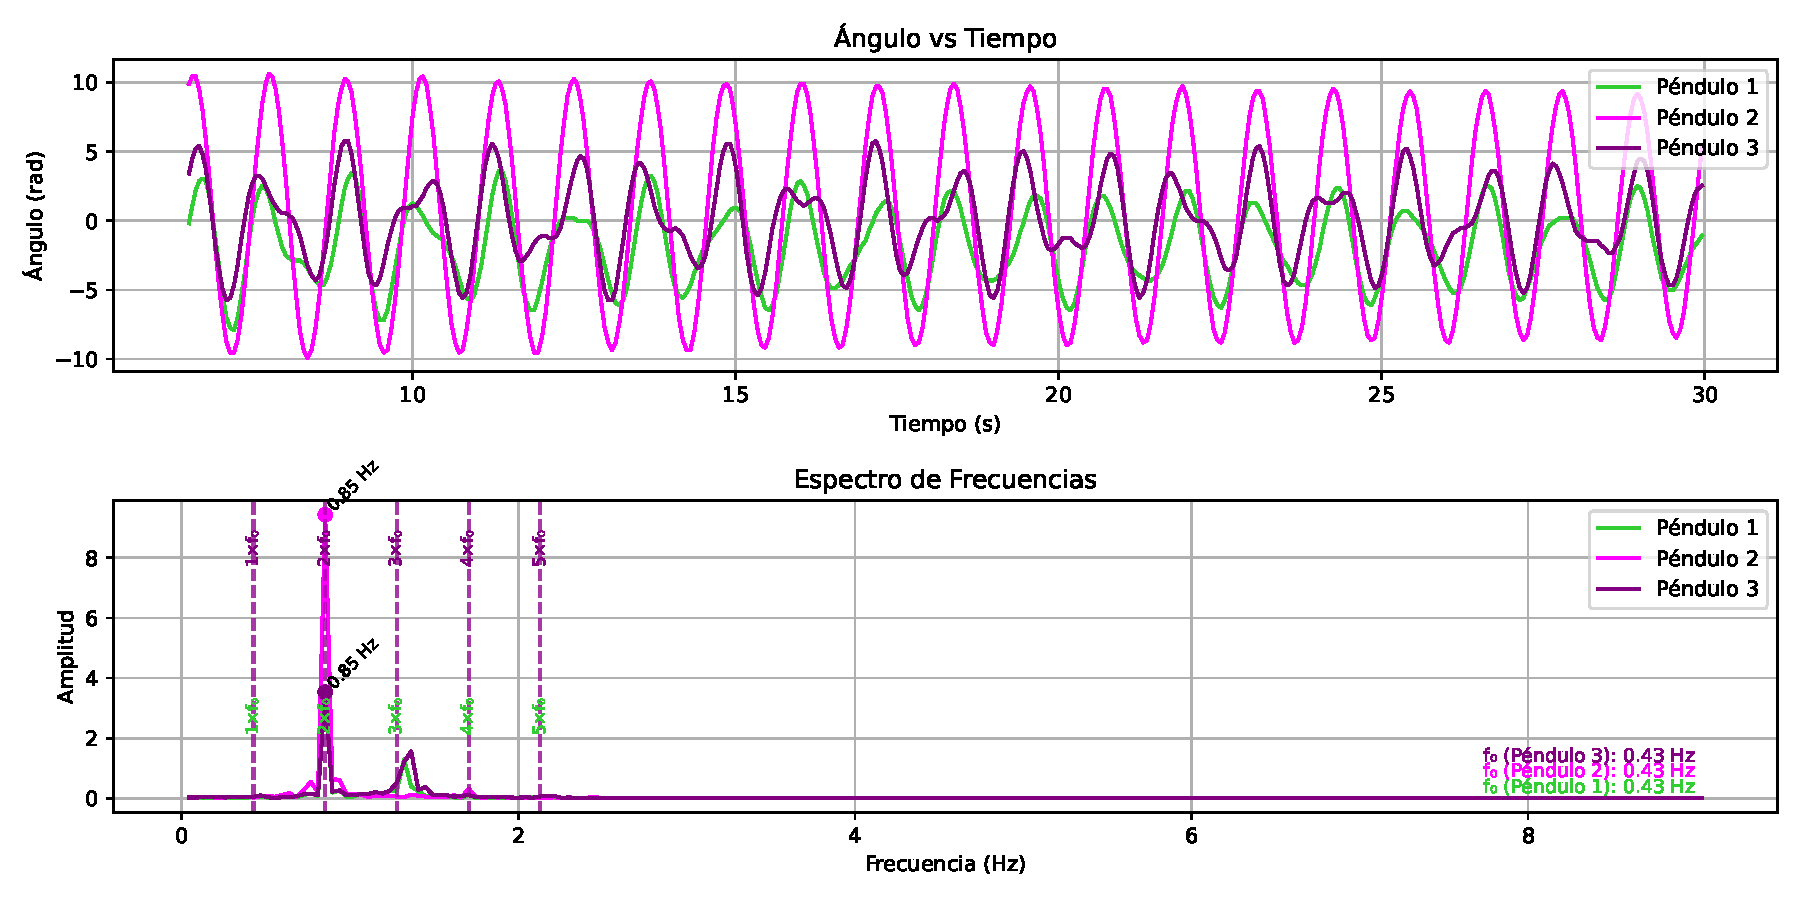
\includegraphics[width=0.8\linewidth]{./Figures/010_66_filtrado.pdf}
    \caption{Evoluci\'on temporal $\theta_i(t)$ y espectro FFT.
        Configuraci\'on 6-6, CI (010).}
    \label{fig:010-66}
\end{figure}

\textbf{An\'alisis de casos espec\'ificos:}

\textbf{\Cref{fig:111-11} (Config. 1-1, CI (111)):}
\begin{itemize}
  \item Cada p\'endulo exhibe un pico de frecuencia principal distintivo en su
    FFT; no comparten una \'unica frecuencia dominante com\'un.
  \item Picos espectrales relativamente anchos: sugiere duraci\'on limitada
    de coherencia o amortiguamiento significativo.
  \item Amortiguamiento esperado: debido a interacciones (acoplamiento,
    fricci\'on) y complejidad del movimiento (laterales desfasados
    respecto al central).
  \item P\'endulo 2: comportamiento temporal con modulaciones en amplitud,
    no arm\'onico simple.
\end{itemize}

\textbf{\Cref{fig:010-51} (Config. 5-1, CI (010)):}
\begin{itemize}
  \item Picos espectrales m\'as definidos y estrechos: comportamiento m\'as
    regular, menos amortiguado para frecuencias dominantes.
  \item Los tres p\'endulos comparten la misma frecuencia principal (reafirma
    tendencia para CI (010)).
  \item Componentes espectrales secundarias comunes, con diferentes
    amplitudes relativas entre p\'endulos.
  \item P\'endulo 3: menor amplitud en componentes espectrales (posiblemente
    menor eficiencia en transmisi\'on de energ\'ia por geometr\'ia de
    acople).
  \item Evoluci\'on temporal m\'as estable y coherente; disminuci\'on gradual
    de amplitudes (amortiguamiento residual).
\end{itemize}

\textbf{\Cref{fig:101-61} (Config. 6-1, CI (101)):}
\begin{itemize}
  \item An\'alisis espectral revela tres picos de frecuencia principales
    distintos (sugiere excitaci\'on de m\'ultiples modos normales).
  \item P\'endulo 3: mayor amplitud en su frecuencia principal y pico
    espectral m\'as estrecho comparado con P1 (relacionado con
    naturaleza del acoplamiento y excitaci\'on inicial de P3).
  \item P\'endulo 2: oscilaciones de amplitud muy reducida (consistente con
    modo normal donde laterales se mueven desfasados y P2 tiene
    participaci\'on m\'inima).
  \item Evoluci\'on temporal: intercambio de energ\'ia entre P1 y P3
    (pulsaciones/batidos), esperado si frecuencias de modos son cercanas
    y hay transferencia de energ\'ia.
\end{itemize}

\textbf{\Cref{fig:010-62} (Config. 6-2, CI (010)):}
\begin{itemize}
  \item P\'endulo 2 (espectro): frecuencia principal con amplitud prominente y
    pico estrecho. Componente secundaria a aprox. $4 f_P$.
    Comportamiento temporal similar a M.A.S.
  \item P\'endulo 1 (espectro): comparte $f_P$ de P2. Otro pico significativo
    a frecuencia $> 3 f_P$. Movimiento no estrictamente M.A.S.,
    pero con clara periodicidad.
  \item P\'endulo 3 (espectro): dos picos con amplitudes comparables,
    frecuencias corresponden aprox. con valores te\'oricos esperados
    (\qty{0.83}{\Hz} y \qty{1.2}{\Hz}). Amplitudes bajas, oscilaci\'on
    de escasa magnitud.
\end{itemize}

\textbf{\Cref{fig:100-66} (Config. 6-6, CI (100)):}
\begin{itemize}
  \item Geometr\'ia de acople facilita transmisi\'on efectiva de energ\'ia.
  \item An\'alisis espectral: los tres p\'endulos comparten componentes de
    frecuencia en mismas ubicaciones espectrales.
  \item P1 y P3 comparten frecuencia principal com\'un (m\'as alta).
  \item P2 tiene su propia $f_P$ (menor), pero exhibe picos secundarios en
    frecuencias donde P1 y P3 oscilan predominantemente (participa en
    modos de mayor frecuencia).
  \item Comportamiento (todos oscilan significativamente) distingue esta
    combinaci\'on, resaltando papel determinante de posici\'on de acoples.
\end{itemize}


\chapter{Discusión}
\label{sec:discusion}

Los resultados experimentales presentados confirman en gran medida los
modelos teóricos. Las figuras de Lissajous y los patrones de enfoque se
corresponden bien con las predicciones para campos uniformes y de
gradiente, respectivamente. Sin embargo, el resultado más revelador es el
desdoblamiento del haz en la configuración mixta, cuyo análisis merece una
discusión aparte y detallada.

\section{Análisis del Desdoblamiento del Haz: Análogo Clásico vs. Efecto Cuántico}
\label{ssec:analisis_desdoblamiento}

La observación de un haz que se desdobla en dos puntos discretos evoca
inmediatamente al célebre experimento de Stern-Gerlach (SG), un pilar de
la mecánica cuántica que demostró la cuantización del espín. A pesar de
esta semejanza visual, una análisis riguroso revela que el fenómeno
observado en este montaje es de naturaleza puramente clásica. A
continuación, se exponen las características fundamentales que impiden
catalogarlo como un efecto SG.

\subsection{La Naturaleza de la Fuerza Dominante}

El argumento más contundente reside en la naturaleza de la partícula y la
fuerza que gobierna su trayectoria. El experimento SG original utiliza
partículas \emph{neutras} (átomos de plata) para aislar la interacción
entre el momento dipolar magnético y el gradiente del campo. La fuerza
responsable de la separación es la fuerza de Stern-Gerlach,
$\boldsymbol{F}_{\text{espín}} = \nabla (\boldsymbol{\mu} \cdot \boldsymbol{B}^*)$.

En nuestro experimento, la partícula es un electrón, una partícula
\emph{cargada}. Como se demostró cuantitativamente en la
\cref{ssec:modelo_spin}, la fuerza de Lorentz que actúa sobre la carga
del electrón es aproximadamente $10^{11}$ veces mayor que cualquier
posible fuerza sobre su espín. Por lo tanto, la dinámica observada es,
casi en su totalidad, el resultado de la fuerza de Lorentz. El desdoblamiento
no proviene de una interacción con el espín, sino de una compleja
interacción de la \emph{carga} del electrón con los campos externos.

\subsection{Campos Dinámicos (AC) vs. Estáticos (DC)}

El experimento SG canónico requiere un campo magnético \emph{estático}
(DC) con un gradiente espacial muy pronunciado y constante en el tiempo.
La separación que produce es, por tanto, estática: los átomos son
desviados permanentemente hacia una de dos trayectorias.

Nuestro montaje, en cambio, se basa fundamentalmente en campos
\emph{dinámicos} (AC) que oscilan a una frecuencia de \qty{50}{\hertz}.
El patrón observado no es una separación estática, sino una \emph{oscilación}
del haz entre dos puntos. El electrón no elige una de dos trayectorias
fijas, sino que es guiado alternativamente a una y otra posición por los
campos que varían en el tiempo. Esta dependencia temporal es ajena al
concepto del experimento SG.

\subsection{Separación Clásica vs. Cuantizada}

La separación en el experimento SG es una manifestación directa de la
\emph{cuantización del espacio}. Para una partícula de espín-1/2, existen
únicamente dos proyecciones de espín posibles, lo que resulta en
exactamente dos haces. La magnitud de esta separación depende de
constantes fundamentales de la naturaleza.

En nuestro experimento, la posición de los dos puntos observados no está
fijada por constantes fundamentales, sino que depende de los parámetros
\emph{clásicos} y continuamente ajustables del sistema: la geometría de
las bobinas, la amplitud y frecuencia de las corrientes, y la energía
inicial del haz. Se postula que la topología del campo mixto crea un
\emph{potencial efectivo} con dos mínimos locales. La posición de estos
mínimos puede ser modificada alterando los voltajes y corrientes, algo
que sería imposible en un desdoblamiento cuántico verdadero.

En conclusión, el fenómeno observado es un fascinante \emph{análogo clásico}
del experimento de Stern-Gerlach. Demuestra cómo una compleja ingeniería
de campos electromagnéticos clásicos y dependientes del tiempo puede
generar un comportamiento que simula visualmente un resultado cuántico. Lejos
de ser una medición del espín, es un testimonio de la riqueza de la dinámica
no lineal en el electromagnetismo clásico.


\printbibliography

\end{document}
